
\documentclass[12pt,a4paper,hidelinks,fleqn]{article}            % Article 12pt font for a4 paper while hiding links
\usepackage[margin=1in]{geometry}                          % Required to adjust margins
../styleAndCommands.tex
\title{\vspace{-5ex}Assignment 3, FE5116 (2014/2015, Semester 2)\vspace{-7ex}}
\date{}
\begin{document}
\maketitle

\subsection*{Excercise 3.1}
 
This excercise considers stock paying pre-defined discrete dividend rates \verb=div_rs= at discrete time \verb=div_ts=. 
\vspace{-1cm}
\paragraph{a)} Implement a function 
\vspace{-5mm}
\begin{verbatim}
europeanBinomialPricerD(spot, sigma, rf, T, N, payoff, div_ts, div_rs)
\end{verbatim}
\vspace{-5mm}
that prices European payoff on this stock using CRR binomial tree.
Unlike the European payoff example code given in the lecture notes that uses the last time step of the tree, 
you are required to calculate the price backward in the tree despite it is more expensive. 
You can use the American put option example pricer as reference for backward pricing.  

Both \verb=div_ts= and \verb=div_rs= are of type array of doubles.
The argument \verb=payoff= is a function from the spot price at expiry to the payoff (same as the example code in the lecture notes). 
The risk free rate \verb=rf= is constant.
When the dividend time does not fall exactly on one time step, 
you can round it to its nearest time step.


For 
\vspace{-1cm} 
\begin{verbatim}
    spot = 100
    sigma = 20%
    rf = 4%
    T = 2
    div_ts = [0.5, 1.0, 1.5]
    div_rs = [5%, 5%, 5%]
\end{verbatim} 
price an European call option with strike = $85$ for different time steps \verb=N= from 10 to 200,
and plot the error against analytic formula. 
The analytic formula for European call option on discrete dividend paying stock is
\begin{align*}
C(S_0, K, T) = e^{-rT} (F N(d_+) - K N(d_-))
\end{align*}
where $N(\cdot)$ is the standard cumulative normal function, and
\begin{align*}
F = S_0 e^{rT} \Pi_i^n (1-\delta_i), ~~
d_{\pm} = \frac{ln\frac{F}{K}  \pm \frac{1}{2}\sigma^2T}{\sigma\sqrt{T}}.
\end{align*}

\paragraph{Solution}
\begin{verbatim}
function v = europeanBinomialPricerD(spot, sigma, rf, T, N, payoff, div_ts, div_rs)
  dt = T / N;
  mu = rf - 0.5 * sigma * sigma;
  # use log S as state variable
  
  # CRR parameters
  a = sqrt(1+ mu * mu / sigma / sigma * dt);
  u = sigma * sqrt(dt) * a;
  d = -u;
  p = 0.5 + mu / 2 / sigma * sqrt(dt) / a;

  # dividend adjustment
  spotadj = spot;
  for k = 1 : length(div_rs)
      spotadj *= 1-div_rs(k);
  endfor
  for i = 1 : (N+1)
      price(i) = payoff( spotadj * exp(2*(i-1)*u - N*u) );
  endfor

  for i = 0:(N-1)
      for j = 1:(N-i)
         price(j) = price(j)*(1-p) + price((j+1))*(p);
      endfor
  endfor
  v = exp(-rf*T) * price(1);
endfunction
\end{verbatim}

\vspace{-1cm}
\paragraph{b)} Extend the function in a) to 
\vspace{-5mm}
\begin{verbatim}
americanBinomialPricerD(spot, sigma, rf, T, N, payoff, div_ts, div_rs)
\end{verbatim}
\vspace{-5mm}
that prices American style options. 
Plot the prices for American call option strike at 85 for N from 10 to 200, and overlay the plot with the plot generated in a). 
Care should be taken that at the dividend paying time, 
the early exercise decision should be made by comparing the continuation value of the option against the intrinsic value calculated from the preferable stock price.
For example, at the dividend time step, the holder of a call option, if decided to exercise, would definitely exercise with the spot price before dividend payment.
Similarly, the holder of a put option would exercise at the spot price after dividend payment.
What about a generic \verb=payoff= function? 

\begin{small}

\begin{verbatim}
function v = americanBinomialPricerD(spot, sigma, rf, T, N, payoff, div_ts, div_rs)
  dt = T / N;
  mu = rf - 0.5 * sigma * sigma;
  # use log S as state variable
  # CRR parameters
  a = sqrt(1+ mu * mu / sigma / sigma * dt);
  u = sigma * sqrt(dt) * a;
  d = -u;
  p = 0.5 + mu / 2 / sigma * sqrt(dt) / a;
  # dividend adjustment
  spotadj = spot;
  for k = 1 : length(div_rs)
      spotadj *= 1-div_rs(k);
  endfor
  df = exp( -rf * dt );
  # terminal
  for i = 1 : (N+1)
      price(i) = payoff( spotadj * exp(2*(i-1)*u - N*u) );
  endfor

  for i = 0:(N-1)
    adj = 1;
    prevDiv = 0; # previous dividend payment time
    for k = 1 : length(div_ts)
    	if ( div_ts(k) <= dt * (N-i) )
        adj *= 1 - div_rs(k);
        prevDiv = k;
	    endif
    endfor
    # also need to check if the current time step is dividend time, 
    # if yes, do a max of payoff(S_before) and payoff(S_after)
    divrate = 0;
    isDivTime = false;
    if prevDiv > 0
      isDivTime = abs (dt * (N-i) - div_ts(prevDiv)) < 0.5 * dt;
      divadj = 1/(1-div_rs(prevDiv));
    endif
    if isDivTime == false && prevDiv < length(div_ts)
      isDivTime = abs (dt * (N-i) - div_ts(prevDiv+1)) < 0.5 * dt;
      divadj = 1-div_rs(prevDiv+1);
    endif
    
    for j = 1:(N-i)
      S = spot * adj * exp(2*(j-1)*u - (N-1-i)*u);
	    pS = payoff(S);
      if isDivTime
        pS = max(pS, payoff(S * divadj));
      endif
	    euro = price(j)*(1-p) + price((j+1))*(p);
      price(j) = max(df*euro, pS);
    endfor
  endfor
  v = price(1);
endfunction
\end{verbatim}
\end{small}

\vspace{-1cm}
\paragraph{c)} For the same test case in a) and time step \verb-N=100-, 
price a European Call, European Put, European Straddle (straddle payoff is $\max(S-K, K-S)$) options with strike = 85. 
Compare the three prices. \\
\emph{For European payoff, Straddle = Call + Put}
\begin{verbatim}
call = 13.315, Put = 6.0434, Straddle = 19.358
\end{verbatim}

\vspace{-1cm}
\paragraph{d)} For the same test case in a) and time step \verb-N=100-, 
price a American Call, American Put, American Straddle options with strike = 85. 
Compare the three prices.
\emph{For American payoff, Straddle $<$ Call + Put}
\begin{verbatim}
call = 18.089, Put = 6.4393, Straddle = 22.862
\end{verbatim}


\paragraph{ex1.m}
\begin{small}
\begin{verbatim}
spot=100; K=85; T=2; N=200; rf=0.04;sigma = 0.2;
div_ts = [0.5, 1.0, 1.5];div_rs = [0.05, 0.05, 0.05];

function res=call(S,K)
  res=max(S-K,0);
end 
function res=put(S,K)
  res=max(K-S,0.0);
end 
function res=straddle(S,K)
  res=max(S-K,K-S);
end 

payoff=@(x)callPayoff(x,K);
euroP=zeros(1,length(10:200));
amerP=zeros(1,length(10:200));
length(euroP)
for i=10:200
   euroP(i-9)=europeanBinomialPricerD(spot, sigma, rf, T, i, payoff, div_ts, div_rs);
   amerP(i-9)=americanBinomialPricerD(spot, sigma, rf, T, i, payoff, div_ts, div_rs);
end 

# analytic price for reference
# dividend adjustment
spotadj = spot;
for k = 1 : length(div_rs)
  spotadj *= 1-div_rs(k);
endfor
F = spotadj * exp(rf*T);
d1 = (log (F/K) + 0.5 * sigma * sigma * T) / sigma / sqrt(T);
d2 = (log (F/K) - 0.5 * sigma * sigma * T) / sigma / sqrt(T); 
bs = exp(-rf*T) * (F * normcdf(d1) - K*normcdf(d2))

plot([10:200],euroP,'g;EuroBinomialCRR;',
     [10:200],amerP,'b;AmerBinomialCRR;',
     [10:200],repmat(bs, 1, length(euroP)),'r;BS Analytic;');
xlabel('Number of time steps');
ylabel('Price');

f=@(x)callPayoff(x,85);
europeanBinomialPricerD(spot, sigma, rf, T, 100, f, div_ts, div_rs)
americanBinomialPricerD(spot, sigma, rf, T, 100, f, div_ts, div_rs)
f=@(x)putPayoff(x,85);
europeanBinomialPricerD(spot, sigma, rf, T, 100, f, div_ts, div_rs)
americanBinomialPricerD(spot, sigma, rf, T, 100, f, div_ts, div_rs)
f=@(x)straddlePayoff(x,85);
europeanBinomialPricerD(spot, sigma, rf, T, 100, f, div_ts, div_rs)
americanBinomialPricerD(spot, sigma, rf, T, 100, f, div_ts, div_rs)
\end{verbatim}

\end{small}

\begin{center}
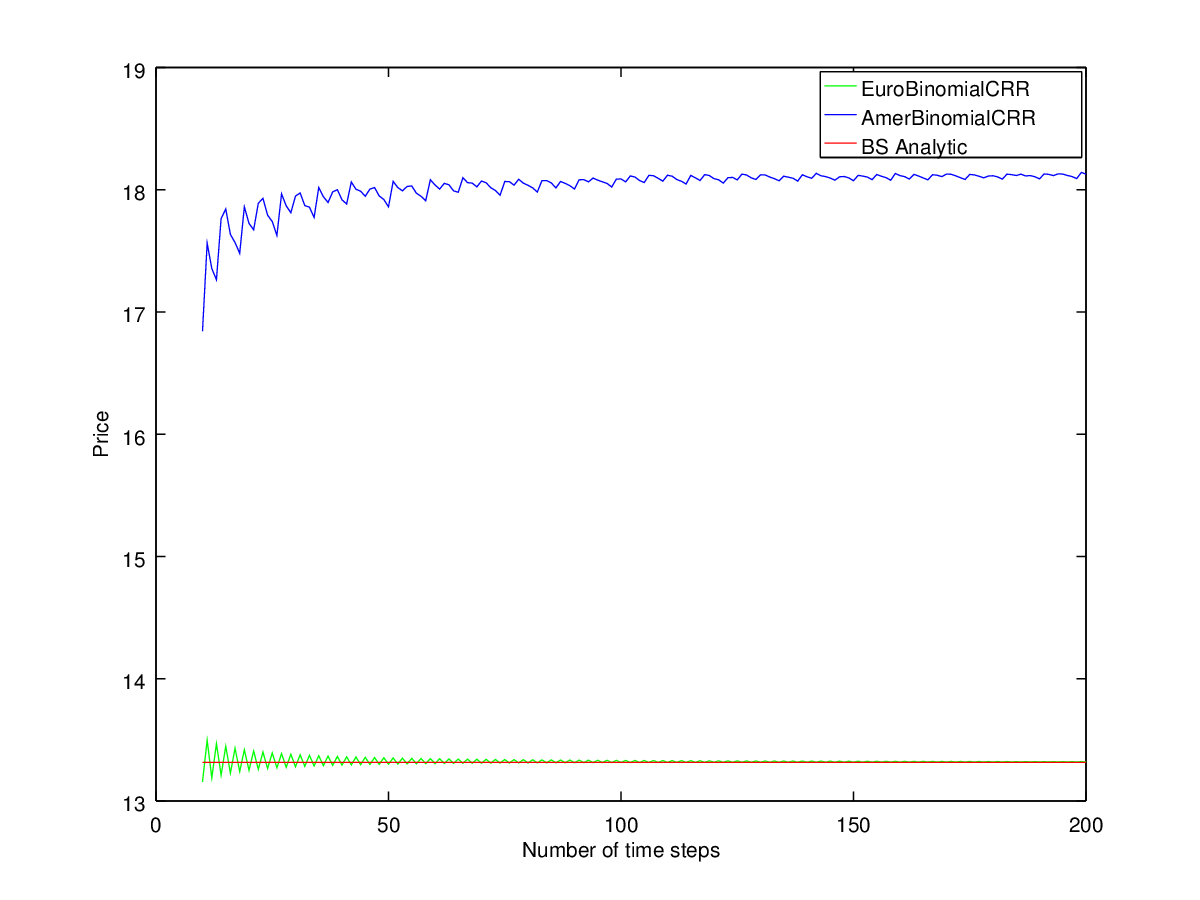
\includegraphics[scale=0.7]{binomialtreePrices}
\end{center}


\subsection*{Excercise 3.2}
Implement two trinomial tree pricers for European options on a dividend-free stock:  
\vspace{-5mm}
\begin{verbatim}
europeanTrinomialPricerCRR(spot, sigma, rf, T, N, payoff)
europeanTrinomialPricerB(spot, sigma, rf, T, N, payoff)
\end{verbatim}
\vspace{-5mm}
where \verb=europeanTrinomialPricerCRR= constructs the tree using combined two steps of CRR binomial tree,
\verb=europeanTrinomialPricerB= uses Boyle '86 ($m=1, ud=1, u = \exp(\sigma\sqrt{2dt})$).

For 
\vspace{-1cm} 
\begin{verbatim}
    spot = 100
    sigma = 20%
    rf = 4%
    T = 2
\end{verbatim} 

Plot the convergence chart (error versus discretization time steps N from 10 to 200) of the two trinomial tree pricers and the CRR binomial tree pricers implemented in Excercise 3.1 a) for call options with K = 70, 90, 110, 130.
The error here refers to the difference between the tree price and the BS analytic price.

\paragraph{Solution}

\begin{verbatim}
function v = europeanTrinomialPricerCRR(spot, sigma, rf, T, N, payoff)
  dt = T / N / 2;
  mu = rf - 0.5 * sigma * sigma;
  # use log S as state variable
  
  # CRR parameters
  a = sqrt(1+ mu * mu / sigma / sigma * dt);
  u = sigma * sqrt(dt) * a;
  d = -u;
  p = 0.5 + mu / 2 / sigma * sqrt(dt) / a;

  for i = 1 : (2*N+1)
      price(i) = payoff( spot * exp(2*u*(i-1-N)) );
  endfor  

  for i = 1:N
      for j = 1:(2*N+1-2*i)
         price(j) = price(j)*(1-p)*(1-p) + 2*price(j+1)*(1-p)*p + price(j+2)*p*p;
      endfor
  endfor
  v = exp(-rf*T) * price(1);
endfunction
\end{verbatim}

\begin{verbatim}
function v=europeanTrinomialPricerB(spot, sigma, rf, T, N, payoff)
  # Bolye parameters
  dt=T/N;
  u=exp(sigma*sqrt(2*dt));
  d=1/u;
  ss = exp((2*rf*T + sigma*sigma*T)/N);
  rr = exp( rf*T / N);
  pu = (ss - (d+1)*rr + d) / ((u-1)*(u-d));
  pd = (ss - (u+1)*rr + u) / ((1-d)*(u-d));
  pm=1-pu-pd;
  for i = 1 : (2*N+1)
      price(i) = payoff( spot * (u^(i-1-N)));
  endfor
  for i = 1:N
      for j = 1:(2*N+1-2*i)
         price(j) = price(j)*pd + price(j+1)*pm + price(j+2)*pu;
      endfor
  endfor
  v = exp(-rf*T) * price(1);  
endfunction
\end{verbatim}

\begin{verbatim}
function ex2(K)
  spot=100; 
  T=2; 
  rf=0.04;
  sigma = 0.2;

  function res=call(spot,strike)
    res=max(spot-strike,0);
  end 
  payoff=@(x)call(x,K);

  # analytic price for reference
  F = spot * exp(rf*T);
  d1 = (log (F/K) + 0.5 * sigma * sigma * T) / sigma / sqrt(T);
  d2 = (log (F/K) - 0.5 * sigma * sigma * T) / sigma / sqrt(T); 
  bs = exp(-rf*T) * (F * normcdf(d1) - K*normcdf(d2))

  p1=zeros(1,length(10:200));
  p2=zeros(1,length(10:200));
  p3=zeros(1,length(10:200));
  for i=10:200
    p1(i-9)=europeanBinomialPricerD(spot, sigma, rf, T, i, payoff, [], []);
    p2(i-9)=europeanTrinomialPricerCRR(spot, sigma, rf, T, i, payoff);
    p3(i-9)=europeanTrinomialPricerB(spot, sigma, rf, T, i, payoff);
  end 

  plot([10:200],p1,'g;EuroBinomialCRR;',
       [10:200],p2,'b;EuroTrinomialCRR;',
       [10:200],p3,'m;EuroTrinomialB;',
       [10:200],repmat(bs, 1, length(p2)),'r;BS Analytic;');
  xlabel('Number of time steps');
  ylabel('Price');
endfunction
\end{verbatim}

\begin{figure}
\begin{tabular}{cc}
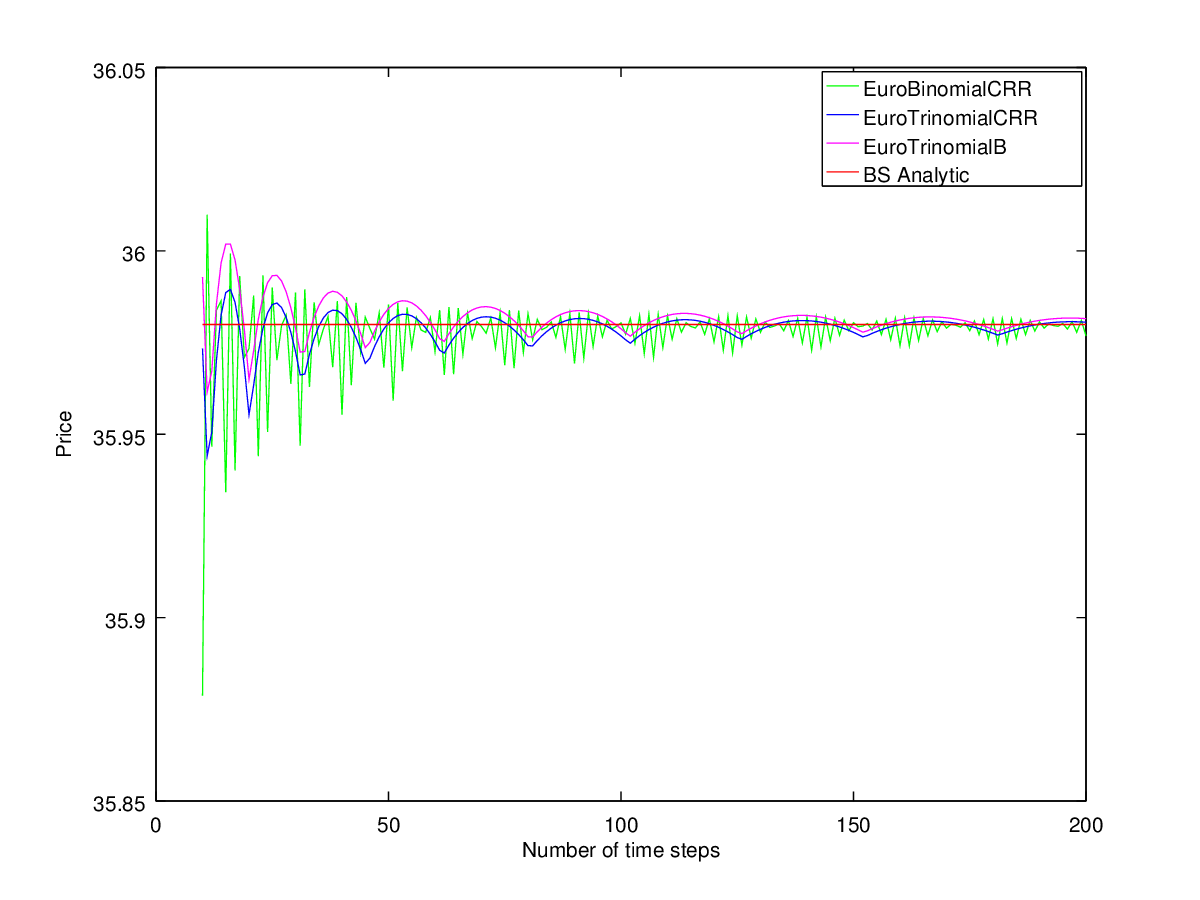
\includegraphics[scale=0.4]{ex2_70} &
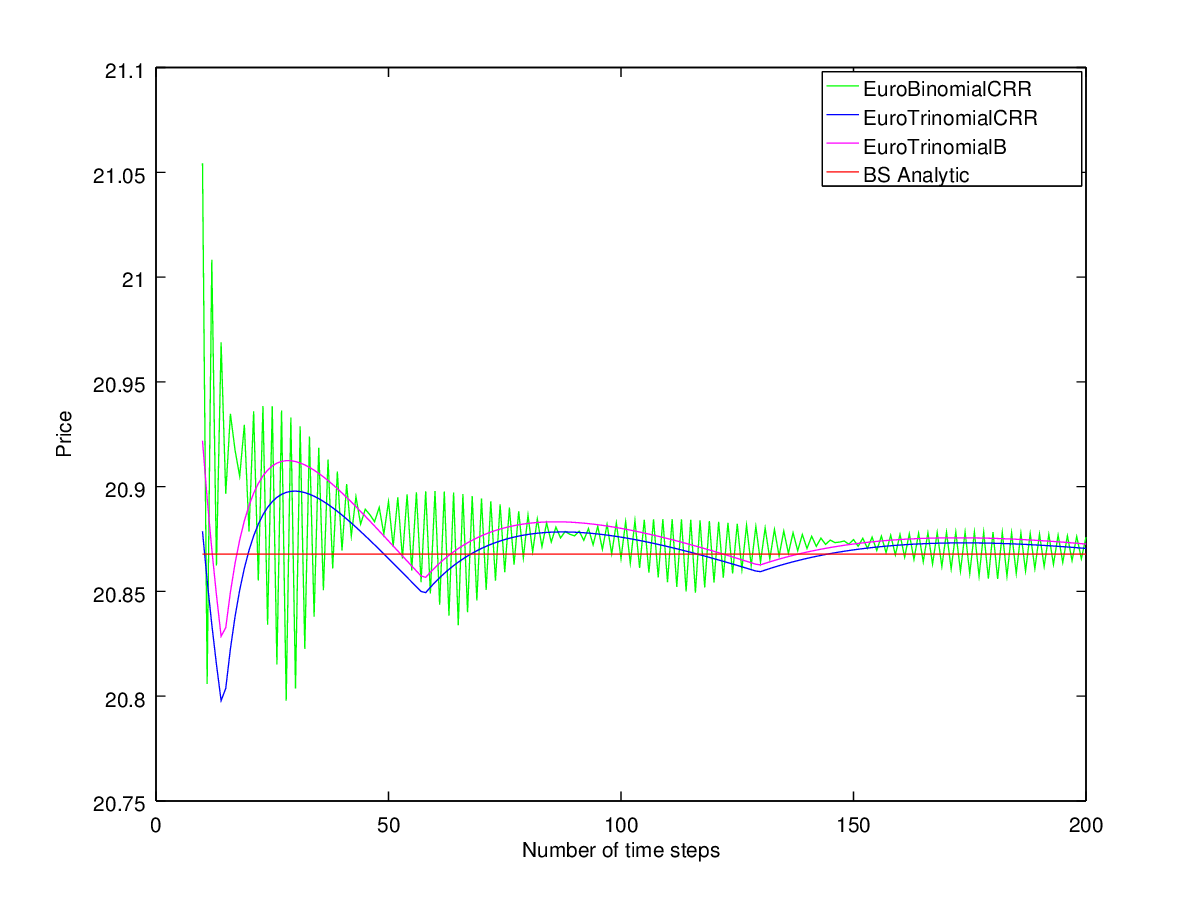
\includegraphics[scale=0.4]{ex2_90} \\
K = 70 & K = 90 \\
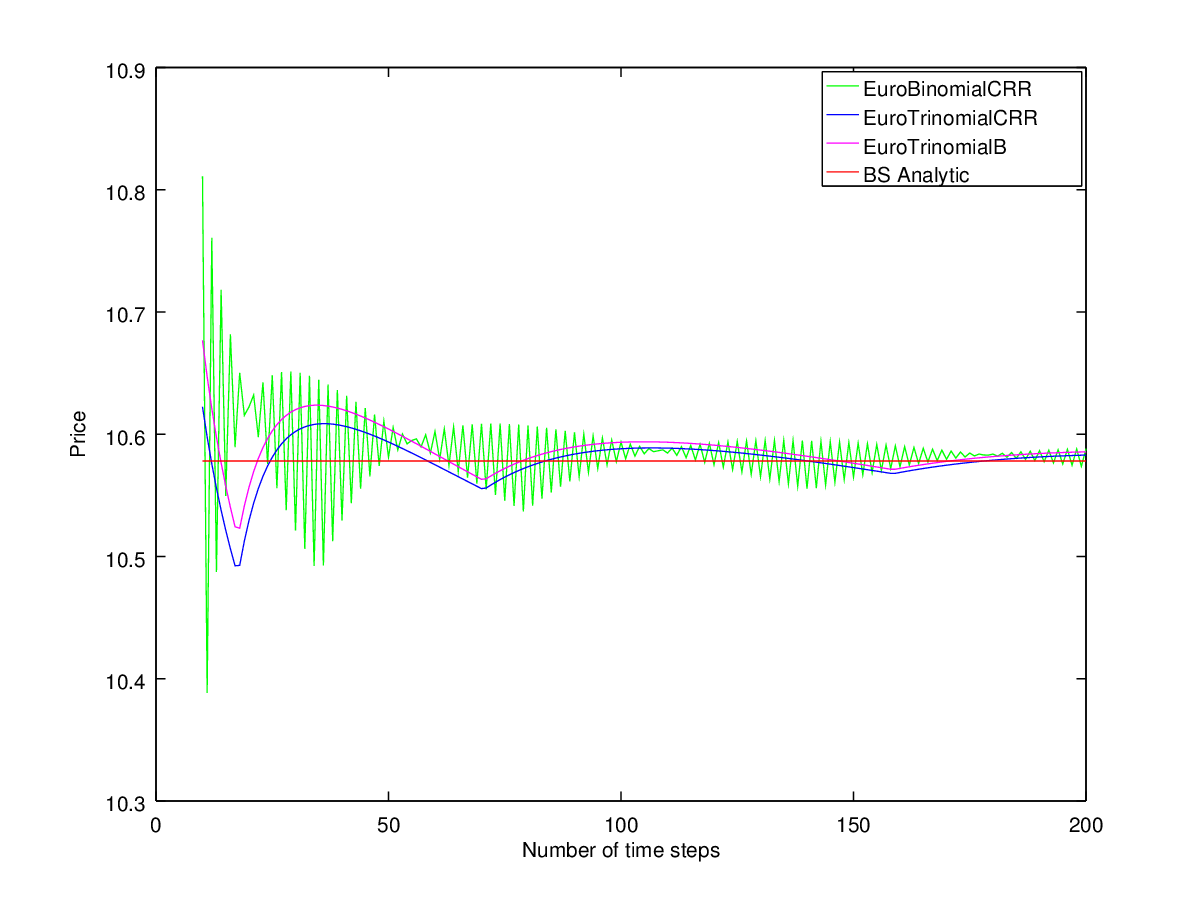
\includegraphics[scale=0.4]{ex2_110} &
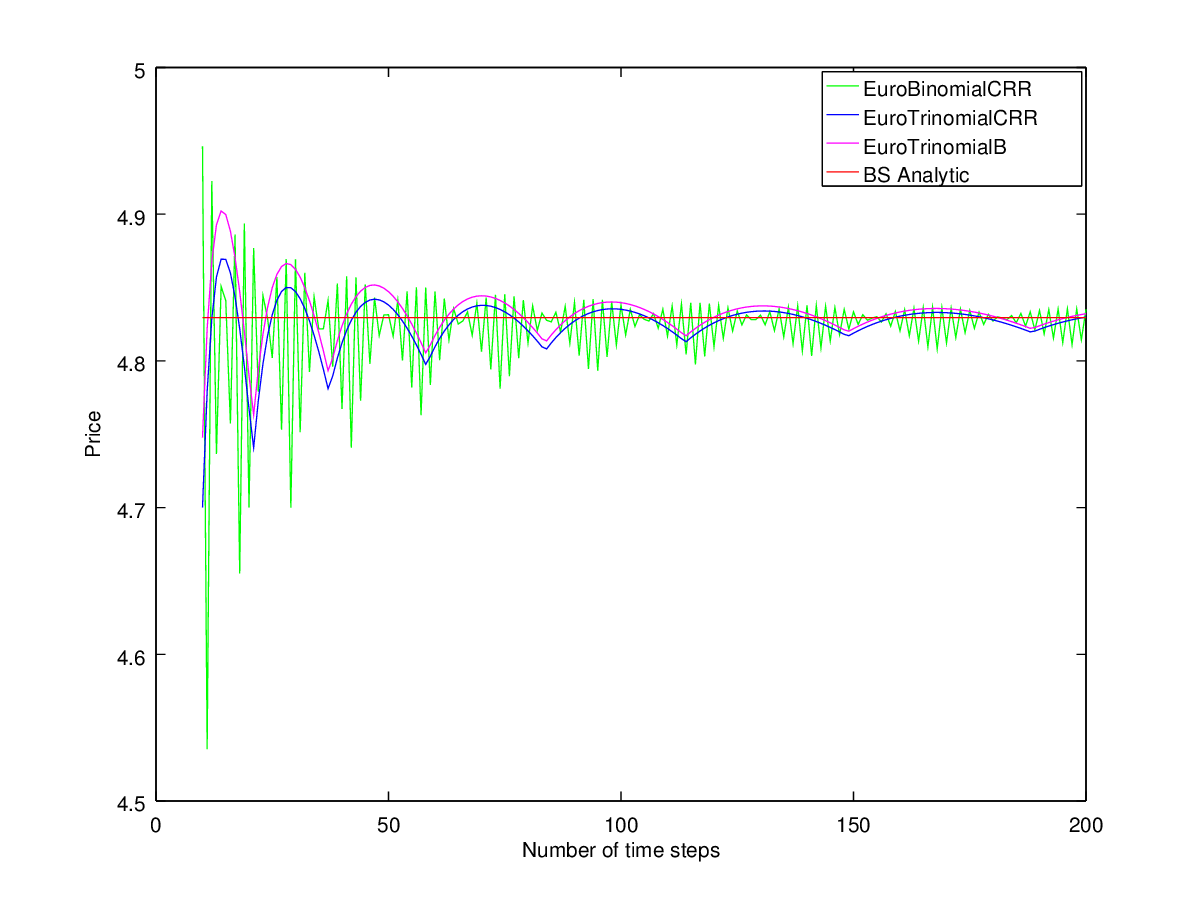
\includegraphics[scale=0.4]{ex2_130} \\
K = 110 & K = 130 \\
\end{tabular}
\end{figure}

\end{document}
